% Licensed to the Apache Software Foundation (ASF) under one or more
% contributor license agreements. See the NOTICE file distributed with
% this work for additional information regarding copyright ownership.
% The ASF licenses this file to You under the Apache License, Version 2.0
% (the ``License''); you may not use this file except in compliance with
% the License. You may obtain a copy of the License at
%
% http://www.apache.org/licenses/LICENSE-2.0
%
% Unless required by applicable law or agreed to in writing, software
% distributed under the License is distributed on an ``AS IS'' BASIS,
% WITHOUT WARRANTIES OR CONDITIONS OF ANY KIND, either express or implied.
% See the License for the specific language governing permissions and
% limitations under the License.

\subsubsection{Sharepoint Job Options}

You must fill in six more tabs to configure a Sharepoint job.

\bigimage{shp-edit-job-tab3}

\ifJDBCGuide
% Licensed to the Apache Software Foundation (ASF) under one or more
% contributor license agreements. See the NOTICE file distributed with
% this work for additional information regarding copyright ownership.
% The ASF licenses this file to You under the Apache License, Version 2.0
% (the ``License''); you may not use this file except in compliance with
% the License. You may obtain a copy of the License at
%
% http://www.apache.org/licenses/LICENSE-2.0
%
% Unless required by applicable law or agreed to in writing, software
% distributed under the License is distributed on an ``AS IS'' BASIS,
% WITHOUT WARRANTIES OR CONDITIONS OF ANY KIND, either express or implied.
% See the License for the specific language governing permissions and
% limitations under the License.

\begin{itemize}
\label{scheduling}

\item \textbf{Schedule type:} Whether you want to scan every document
once or dynamically recrawl content in your repository. 

When scanning every document once, the crawler marks all documents that
have been previously crawled in this job as potentially to be deleted,
adds all seed documents to its queue and marks them as pending, processes
pending documents, marking them completed as they are ingested, and then
deleted all of the documents that were not recrawled. A document might
not be recrawled because it no longer exists, or the job specification
might have been changed to no longer include the document.

When dynamically recrawling documents, the crawler does not start by
marking all documents as potentially deletable; instead, it begins with
all of the seed documents, and continues adding to its list, periodically
re-adding the initial seed documents. If a document is removed from the
source, it will expire in the expiration interval (see below).

\item \textbf{Expiration Interval (if continuous):} The length of the
interval (in minutes) that the appliance will retain a document
crawled by this job after the document no longer appears in the
repository. After this interval, the missing document will be removed
from the appliance's index and archive. Leave the expiration interval
blank to keep missing documents indexed in GTS.

\item \textbf{Recrawl interval:} If you are dynamically recrawling
documents, how long, in minutes, the crawler should wait before
crawling documents a second time.

\item \textbf{Reseed interval:} If you are dynamically recrawling
documents, how long, in minutes, the crawler should wait before
looking for new documents to crawl. \ifMeridioGuide This connector
identifies all documents for ingestion through seeding; if the reseed
interval is infinite, the job will not ingest documents placed in the
repository during run time. (The job automatically reseeds whenever it
is started.) The default interval of 60 minutes is an appropriate
reseed rate. \fi \ifFilenetGuide This connector identifies documents
for ingestion during seeding. If you change the document inclusion
criteria, reseeding is required to identify new documents. Similarly,
documents placed in the repository while the job is running will not
be identified until the crawl is reseeded.  (The job automatically
reseeds whenever it is started.) The default interval of 60 minutes is
an appropriate reseed rate. \fi

\item \textbf{Scheduled time:} Allows you to define a time you wish
the job to run using a series of selection boxes. The first box refers
to the day of the week you wish the job to run, with an option to have
the job run any day of the week. The second box allows you to select
the start hour, with an option to start the job at any hour. The third
box allows you to specify which minute after the hour that you wish
the job to start. The fourth box allows you to specify what months of
the year you wish the job to run, with an option for the job to run
any month. The last box allows you to specify the day of the month you
wish the job to start, including any day of month.


You can scroll through each of the five boxes in this setting using
the arrow keys on your keyboard or by using the scroll bar on the
right side of the box.  If you want to select more than one value,
hold down control as you scroll and click the values that you want to
select. This allows you to define multiple windows with the same
length, for example by selecting Monday, Wednesday, and Friday at the
same time.

\item \textbf{Maximum run time:} The longest you will allow the job to
run, in minutes. For example, if you want to start a job at 2 AM but
force it to stop at 8 AM so that users have access to the repository,
you should set this value to 360 minutes. If the job is not complete by the
end time, documents that have already been found will be indexed, and
the rest of the crawl will continue at the beginning of the next
schedule interval. 

When you have defined the scheduled time and assigned a maximum run
time, click on the ``Add Scheduled Time'' button. A new schedule box
will appear below the scheduled time, allowing you to create
additional scheduled run times.

Here is a sample schedule for a job that will run every
Monday from 2 am to 6 am:

\begin{changemargin}{-.3in}{0in} 
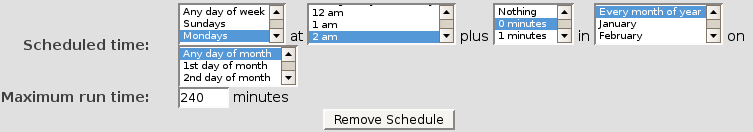
\includegraphics[width=300pt]{sample-schedule}
\end{changemargin}

If you do not have at least one scheduled time, the job will
only run when run manually (see page \pageref{ManageJobs}), and will
not automatically update the index on the appliance based on changes
to the repository.

You can remove a scheduled time by clicking the ``Remove Schedule''
button.

\end{itemize}

\fi

\ifCombinedConnectorGuide
This tab presents scheduling options. Here you can generate one or
more scheduled run times for the job. For a complete description of
the scheduling options, see the description starting on page
\pageref{scheduling}.
\fi

\bigimage{shp-edit-job-tab4}

\begin{itemize}


% I want to do more with the second and third sentences there, but
% I am not seeing a better way either at the moment. :/
\item \textbf{Path rules:} \label{pathrules}
Path rules allow you to include or exclude
subsites, libraries, and files from your crawl. From the point of view
of this tool, a Sharepoint file path has two parts. The first is the
server and site path specified during the creation of the repository
connection, and the second is the location of the file inside that
site. For example, the file path of a given file may be

\begin{changemargin}{-1.5in}{0in}\dirpath{http://server.example.com/SampleSite/Subsite/Library/Folder/file}
\end{changemargin}

You already specified the first part of the path,
\dirpath{http://server.example.com/SampleSite}, when you created the
repository connection. You must now specify subsite, library, folder,
and file information in the path tool. At minimum, you must specify
containing library and file name information in order to crawl any
documents.

% Malima, I think I am tightening this up, can you make sure I am not
% changing any facts by accident? Thanks!

The paths tool has
three sections. At the top, the paths tool displays inclusion and 
exclusion rules that you have already created and added to your
crawl. At the left of the rules are buttons that allow you to delete a
rule, insert a new rule at any place in the list, and add a new rule
to the end of the list. Inclusion/exclusion rules are applied in
order; rules at the top of the list supersede rules further down the
list.

The second section displays the path rule currently being created. The
path match is displayed, as is the rule type. The rule type indicates
if the rule is to be applied to a site, a library, or files. If the
rule includes a text match portion, you will need to select a type. At
the right of this section, you can choose whether the rule you are
creating will be an inclusion or exclusion rule. To add or insert the
displayed rule into the list of path rules, use the appropriate
``Add new rule'' or ``Insert new rule'' button to the left of the
rules list in the first section.
%What does "The appropriate button" mean?  I couldn't tell.

The third section allows you to select sites and libraries and to add
wildcard text matching that will be used in a rule. The
crawler automatically discovers subsites and libraries when the
connection used for a job is working properly. To select a subsite or library
to add to the path rule, simply select it from the appropriate
selection box and click the accompanying add button. To create a match
expression, enter a wildcard match expression in the text box at the
right, and click the ``Add Text'' button. When you add a match
expression, you must then select the match type in the second section
of the path tool. The wildcard expression you entered can be used to
match files, sites, or libraries. To change the rule under
construction, you can click the ``Reset Path'' button to clear the
path rule, or, if applicable, the minus button to remove the last step
of the path rule. The minus button only appears when the last step of
the path rule shown is a Site or Library selection.


\end{itemize}


Initially, no path rules are in place, and, thus, no documents will be
crawled by the job. To include everything in your system, you will need to create a set of rules that include all sites, libraries, and files.

At the top of the list, create a rule that includes all sites. In the
third section of the tool, enter the match expression \texttt{*} in
the text field and click the ``Add text'' button. In the second
selection, select the type ``Site'' and the ``include'' indicator,
then click the ``Add new rule'' button in the top section. This will
add the new rule including all subsites.

Next, create a new rule including all libraries by using the match
expression \texttt{*}, the ``Library'' type, and the ``include''
indicator. Use the ``Add new rule'' button to add it to the bottom of
the list.

Finally create a file rule using, \texttt{*}, ``File'', and
``include'' and add it to the bottom of the list.

This set of rules, shown below, will include all subsites, libraries, and files
accesible from the base site of the crawl.

\bigimage{shp-edit-job-tab4a}

Wildcard expression matching can be very useful for creating more
complicated rules. For example, you might wish to create a rule that
excluded all libraries including the word ``Test'' from a
given subsite, ``SubSite.'' Using the third section of the paths
tool, you would first select ``SubSite'' in the site selection box
and click ``Add Site.'' Then you would type the expression
\texttt{*Test*} in the text box and click the ``Add Text'' button. 
You would select the type ``Library'' and action ``exclude'' in the
second section, as shown below:

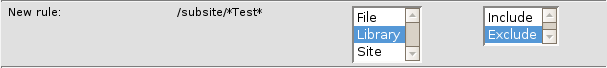
\includegraphics[width=300pt]{shp-edit-job-tab4b}


Click the ``Insert New Rule'' button at the top of the list of rules. This
creates a new rule that excludes
any Library from the subsite ``SubSite'' including the expression
``test'' or ``Test'' in its name. Because this rule is at the top of the list, it will superceed the inclusion rules further down in the list.

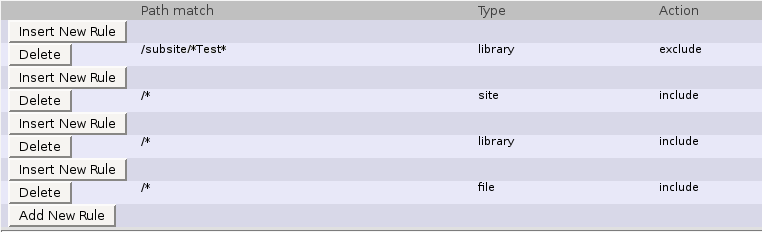
\includegraphics[width=300pt]{shp-edit-job-tab4c}



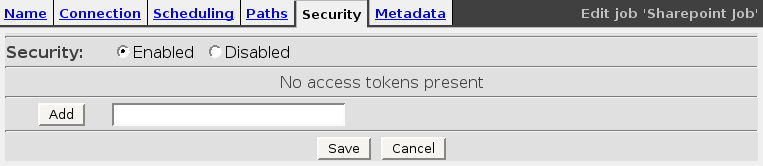
\includegraphics[width=300pt]{shp-edit-job-tab5}

\begin{itemize}

\item \textbf{Security:} Select ``Enabled'' to use Active Directory permissions with the ingested documents. You can configure custom permissions using the ``Access Tokens'' tools, or accept the ACLs as given in the Sharepoint repository. Select ``Disabled'' to allow all document search users to access to the files ingested by this job.

\item \textbf{Access Tokens:} This field allows you to create custom ACLs for the files ingested by this job. Enter the SID of a user or group that you wish to add to the custom ACLs for documents from this job, then click the ``Add'' button. You can continue to add more SIDs. These SIDs will appear in a list. Click the ``Delete'' button next to any SID to remove it from the list.

\end{itemize}


\bigimage{shp-edit-job-tab6}

\begin{itemize}

\item \textbf{Metadata rules:} Using this tool, you can create inclusion and exclusion rules to determine what metadata from the Sharepoint server is ingested with documents crawled by this job. This tool operates in a similar manner to the path rules tool, discussed on page \pageref{pathrules}. The first section displays the list of rules and allows you to delete current rules and add or insert new rules. The second section shows the rule you are currently building. The third section contains tools to insert site, library, and regular expression matching information into the current rule.

To create a metadata rule, you create an inclusion or exclusion rule
in the same fashion as a path rule. In the case of exclusion, all
subsites, libraries, or files specified by your path rule will be
ingested without metadata. For inclusion, you can select to have all
metadata included with the subsites, libraries, or files specified by
your rule, or, in the case of libraries, select individual metadata
fields to be ingested. Highlight individual fields by clicking,
multiple fields by clicking while holding the ``Ctrl'' key, or ranges
of fields by clicking while holding the ``Shift'' key.

As in the case of the path rules, the rules are applied in order from
the top of the list to the bottom. By default, no system metadata is
included. To create a rule to include all metadata, select ``include''
and check the ``Include all metadata'' box in the second section of
the tool, then click the ``Add new rule'' button. The default path is
the base path, so the new rule will instruct the crawler to collect
all metadata for all files crawled through this job.

\item \textbf{Path metadata:} This tool allows you to create a metadata attribute based on URL path data. You can use regular expressions to manipulate the URL. First, enter the name for your path metadata attribute. In the example shown, the attribute is called ``pathdata''. If you do not provide any regular expression mappings, the path metadata will just be the document's path information, not including the path information from the base site of your crawl. For example, the path metadata for a file ``sample'' in a library ``Example'' on the base site of your crawl would be ``/Example/sample''. In this case, all files will have unique values for this metadata attribute.

In the example shown above, the path metadata is manipulated by using
the match expression \texttt{(.*)/(.*)\$} and the replace expression
\texttt{\$(1)}. This mapping strips the file name from the path
metadata, leaving just the site, library, and folder information in
the attribute. For more information on regular expressions, see the
descriptions and note in the path rules section starting on page
\pageref{pathrules}.

To add a mapping, enter a match expression in ``Match regexp'' field
and the replacement expression in the ``Replace string'' field, then
click the ``Add Path Mapping'' button. The mappings are performed in
order from the top of the list down. To remove a mapping from the
list, simply click the ``Delete Path Mapping'' button to its left.


\note{If you are not familiar with regular expressions, there
are a variety of tutorials available on the web, including
\url{http://gnosis.cx/publish/}\linebreak\url{programming/regular_expressions.html}
and \url{http://perldoc.}\linebreak\url{perl.org/perlrequick.html}. If
you still have difficulty with these settings, please contact Customer
Support (see page \pageref{SupportContact}).}


\end{itemize}

After entering this information, you will be taken to the status page
for this job:

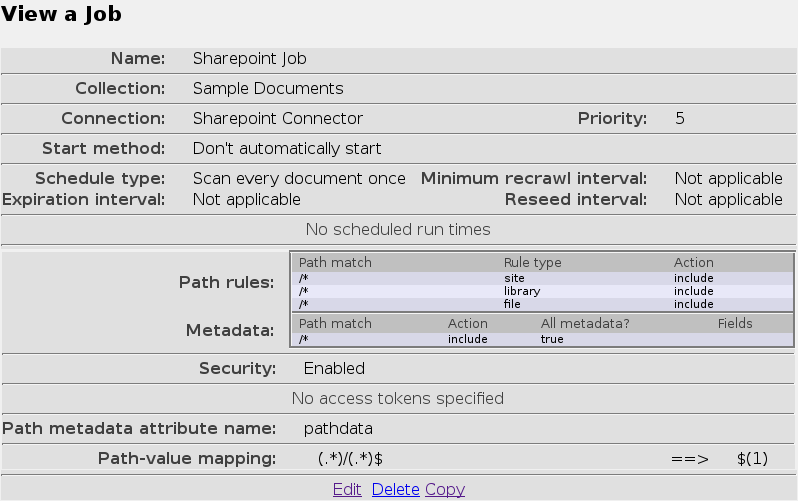
\includegraphics[width=300pt]{shp-view-job-status}
